%%%%%%%%%%%%%%%%%%%%%%%%%%%%%%%%%%%%%%%%%%%%%%%%%%%%%%%%%%%%
%%% LIVECOMS ARTICLE TEMPLATE FOR BEST PRACTICES GUIDE
%%% ADAPTED FROM ELIFE ARTICLE TEMPLATE (8/10/2017)
%%%%%%%%%%%%%%%%%%%%%%%%%%%%%%%%%%%%%%%%%%%%%%%%%%%%%%%%%%%%
%%% PREAMBLE
\documentclass[9pt,tutorial]{livecoms}
% Use the 'onehalfspacing' option for 1.5 line spacing
% Use the 'doublespacing' option for 2.0 line spacing
% Use the 'lineno' option for adding line numbers.
% Use the "ASAPversion' option following article acceptance to add the DOI and relevant dates to the document footer.
% Use the 'pubversion' option for adding the citation and publication information to the document footer, when the LiveCoMS issue is finalized.
% The 'bestpractices' option for indicates that this is a best practices guide.
% Omit the bestpractices option to remove the marking as a LiveCoMS paper.
% Please note that these options may affect formatting.

\usepackage{lipsum} % Required to insert dummy text
\usepackage[version=4]{mhchem}
\usepackage{siunitx}
\DeclareSIUnit\Molar{M}
\usepackage[italic]{mathastext}
\graphicspath{{figures/}}

\usepackage{listings}

%%%%%%%%%%%%%%%%%%%%%%%%%%%%%%%%%%%%%%%%%%%%%%%%%%%%%%%%%%%%
%%% IMPORTANT USER CONFIGURATION
%%%%%%%%%%%%%%%%%%%%%%%%%%%%%%%%%%%%%%%%%%%%%%%%%%%%%%%%%%%%

\newcommand{\versionnumber}{1.3}  % you should update the minor version number in preprints and major version number of submissions.
\newcommand{\githubrepository}{\url{https://github.com/myaccount/homegithubrepository}}  %this should be the main github repository for this article

%%%%%%%%%%%%%%%%%%%%%%%%%%%%%%%%%%%%%%%%%%%%%%%%%%%%%%%%%%%%
%%% ARTICLE SETUP
%%%%%%%%%%%%%%%%%%%%%%%%%%%%%%%%%%%%%%%%%%%%%%%%%%%%%%%%%%%%
\title{This is the title [Article v\versionnumber]}

\author[1*]{Firstname Middlename Surname}
\author[1,2\authfn{1}\authfn{3}]{Firstname Middlename Familyname}
\author[2\authfn{1}\authfn{4}]{Firstname Initials Surname}
\author[2*]{Firstname Surname}
\affil[1]{Institution 1}
\affil[2]{Institution 2}

\corr{email1@example.com}{FMS}  % Correspondence emails.  FMS and FS are the appropriate authors initials.
\corr{email2@example.com}{FS}

\orcid{Author 1 name}{AAAA-BBBB-CCCC-DDDD}
\orcid{Author 2 name}{EEEE-FFFF-GGGG-HHHH}

\contrib[\authfn{1}]{These authors contributed equally to this work}
\contrib[\authfn{2}]{These authors also contributed equally to this work}

\presentadd[\authfn{3}]{Department, Institute, Country}
\presentadd[\authfn{4}]{Department, Institute, Country}

\blurb{This LiveCoMS document is maintained online on GitHub at \githubrepository; to provide feedback, suggestions, or help improve it, please visit the GitHub repository and participate via the issue tracker.}

%%%%%%%%%%%%%%%%%%%%%%%%%%%%%%%%%%%%%%%%%%%%%%%%%%%%%%%%%%%%
%%% PUBLICATION INFORMATION
%%% Fill out these parameters when available
%%% These are used when the "pubversion" option is invoked
%%%%%%%%%%%%%%%%%%%%%%%%%%%%%%%%%%%%%%%%%%%%%%%%%%%%%%%%%%%%
\pubDOI{10.XXXX/YYYYYYY}
\pubvolume{<volume>}
\pubissue{<issue>}
\pubyear{<year>}
\articlenum{<number>}
\datereceived{Day Month Year}
\dateaccepted{Day Month Year}


%%% Shortcuts and macros
\newcommand{\dgsolv}{\Delta G_\textup{solv}}
\newcommand{\software}{\emph}
\newcommand{\todo}{\textcolor{red}}

\lstset{
	basicstyle=\ttfamily\footnotesize
}
\lstdefinestyle{code}{}
\lstdefinestyle{python}{
	language=Python,
	stringstyle=\color[rgb]{1.0, 0, 0},
	commentstyle=\color[rgb]{0, 0, 0.6}
}
\lstset{style=code}

\DeclareSIUnit{\calorie}{cal}
\DeclareSIUnit{\kcalPerMolASqr}{\kilo\calorie\per\mole\per\angstrom\squared}

%%%%%%%%%%%%%%%%%%%%%%%%%%%%%%%%%%%%%%%%%%%%%%%%%%%%%%%%%%%%
%%% ARTICLE START
%%%%%%%%%%%%%%%%%%%%%%%%%%%%%%%%%%%%%%%%%%%%%%%%%%%%%%%%%%%%

\begin{document}

\begin{frontmatter}
\maketitle

\begin{abstract}
Grid inhomogeneous solvation theory (GIST) is a method to compute the free energy of hydration of a compound on a 3-dimensional grid.
The high spatial resolution of the GIST output, as well as the decomposition into energy and entropy contributions, allow for highly detailed analyses on both proteins and small molecules. However, this versatility also comes with a higher entry barrier for new users.

In this tutorial, we aim to guide the reader through the most common steps involved in a GIST analysis at the example of the streptavidin-biotin complex.
Furthermore, we discuss the theory of GIST with a focus on practical aspects, and show several pitfalls and technical difficulties that may occur during a GIST study.
We assume familiarity with molecular dynamics (MD) simulations as well as the AmberTools package.

%This particular document provides a skeleton illustrating key sections for a Tutorial document.
%Please see the sample \texttt{sample-document.tex} in \url{github.com/livecomsjournal/article_templates/templates} for additional information on and examples of using the LiveCoMS LaTeX class.
%Here we also assume familiarity with LaTeX and knowledge of how to include figures, tables, etc.; if you want examples, see the sample just referenced.
%
%In your work, in this particular slot, please provide an abstract of no more than 250 words.
%Your abstract should explain the main contributions of your article, and should not contain any material that is not included in the main text.
%Please note that your abstract, plus the authorship material following it, must not extend beyond the title page or modifications to the LaTeX class will likely be needed.
\end{abstract}

\end{frontmatter}




\section{Introduction}
\todo{ (vah) Sources and better description of all these methods, more literature research, better flow }


Solvation thermodynamics govern any process involving solutes in a solvent.
Solutes are constantly interacting with solvents in their environment, necessitating a good description of these interactions for accurate computational predictions. 
Especially the interaction with water is of utmost importance, as many biological processes occur in a aquaeous environment. 
The free energy of solvation thereby strongly influences real-world problems of interest such as hydrophobic effects, the binding of a ligand to a protein, protein-protein interactions, protein dynamics or even more generally, a protein's fold. 
The computational calculation of thermodynamical solvation properties is therefore of particular interest and has been tackled by a wide array of different methods.   
Quantum mechanical methods provide the most rigorous description of the underlying potential energy surface (PES) but suffer from high computational cost, allowing only the treatment of small systems and few solvent molecules. 
More recently, machine learning approaches and QM/MM approaches are trying to bridge the gap to computationally less demanding methods while keeping the accuracy of ab initio QM methods.
Molecular mechanics based approaches describe the underlying PES through empirically fit force-fields, which reduce the computational demand of these calculations tremendously.
This allows for the treatment of even large biological systems like fully solvated proteins. 
Implicit solvent methods such as MM/PBSA  or MM/GBSA can quickly provide results for a large amount of supplied structures, but yield inaccurate results when compared to more rigorous explicit solvent methods. Somewhat inbetween the implicit solvent methods and the fully explicit solvent methods are Reference Interaction Site Models. One of these methods, 3D-RISM, foregoes the explicit simulation and uses 3D solvent distributions based on the Ornstein--Zernike integral equations to predict solvation thermodynamics instead.
The 3D-RISM approach allows for a decomposition into entropic and enthalpic terms as well as a full localization of the underlying distributions to the solute structure.
The most statisticaly rigorous of the explicit solvent MM methods are alchemical methods such as FEP or TI. 
Assuming sufficient sampling, they can accurately predict the free energy of solvation in the boundaries of the assumptions underlying their forcefield. 
However, the seperation of enthalpic and entropic contributions to the free energy of solvation is difficult with these methods and localizing these contributions not easily possible.
In this tutorial, the Grid Inhomogenous Solvation Theory (GIST) is applied to calculate solution thermodynamic properties of interest. 
GIST is based on Lazaridis' Inhomogenous Solvation Theory (IST), solving the arising integral equations on a grid. 
This is highly advantegous compared to other IST-based methods such as e.g. WaterMap,\todo{Add more methdods!} as this is not restricted to high-occopancy solvation sites but provides a 
By simulating the dynamics of a solvent around the solute, GIST calculates thermodynamic properties for a standard solvation process as described by Ben-Naim.
The method allows for a full localization of entropic and enthalpic contributions on the grid around the solute.
For small organic molecules in water, the method provided results compareable to TI in accuracy, assuming some small correction factor to the entropy is applied. 
Recent improvements to the method have improved the calculation speed tremendously, allowing for the treatment of larger systems of biological interest such as proteases or antibodies. 
Other improvements worked on decreasing differences in the treatment of long-range interaction energies between GIST and popular molecular dynamics engines. 
Yet further changes allow the inclusion of other rigid solvents than water or allow for the treatment of solvent mixtures and ions in solution. 
While previous tutorials gave insightful pointers as to how to setup and run GIST calculations, the post-processing of such calculations was often treated less rigorously. While building on these tutorials, an updated guide to calculating solvation properties using GIST is therefore presented here to address the recent improvements to the method.

%Here you would explain what problem you are tackling and briefly motivate your work.
%
%In this particular template, we have removed most of the usage examples which occur in \texttt{sample-document.tex} to provide a minimal template you can modify; however, we retain a couple of examples illustrating more unusual features of our templates/article class, such as the checklists, and information on algorithms and pseudocode.
%
%Keep in mind, as you prepare your manuscript, that you should plan for a representative image  which will be used to highlight your article on the journal website and publications. Usually, this would be one of your figures, but it must also be uploaded separately upon article submission. We give specific guidelines for this image on the journal website in the section on article submission (see \url{https://livecomsjournal.github.io/authors/policies/index.html#article-submission}).
%
%Additionally, for well-formatted manuscripts, we recommend that you let LaTeX handle figure/table placement for you as much as possible, so please avoid specifying strenuous float instructions like `[h!]` and `[H]` as much as possible.

\subsection{Scope}

The tutorial provides an example of a GIST workflow that can be easily adapted towards different systems. 
In addition to a short introduction to the method and the theory behind it an overview of the various different flavours of GIST methods is provided.
Towards this, a GIST study of the streptavidin-biotin complex is presented, which reflects on many common aspects of GIST studies.
We present solvation analysis of a small molecule (biotin) as well as a biomolecule (streptavidin).
For both systems, we show how to interpret the three-dimensional contributions of solvation free energy in a binding pocket.
The contribution of solvation free energy to binding is computed, which requires accurate post-processing of the GIST output to avoid unfavorable summation of bias in the GIST calculation.
We believe that this example study covers a wide range of applications of the GIST method.
Furthermore, we discuss several technical aspects  and typical pitfalls of GIST analyses, such as the normalization of voxel values and how to deal with double counting of energy contributions. 
Additionally, we provide a python library to unify the analysis of GIST data produced by various versions of GIST and make the post-processing of GIST results more accessible.

After completing this tutorial, we expect the reader to be able to implement their own GIST study. 

%Tutorials should endeavor to cover the specific task at hand, and also highlight how the steps might need to be modified (or additional care might need to be taken at particular points) to handle more general cases.
%
%The scope of the tutorial, as well as the expected proficiencies / outcomes for researchers who complete the tutorial, should be clearly defined.
%This will often happen in a specific section or subsection in the article itself.

\section{Prerequisites}
\todo{ (vah)  Improve flow and logical progression of prerquisites.}

%Here you would identify prerequisites/background knowledge that are assumed by your work, as well as any software/license requirements.

\subsection{Background knowledge}
This tutorial is aimed at advanced users with a solid background knowledge of molecular dynamics (MD) simulations. The user should be able to run MD simulations and work with their output data.
Previous knowledge of the method is not necessary, but we recommend the perusal of the primary sources on the method outlined in the Theory section. 

The presented analyses are run in Python.
A working understanding of Python is therefore necessary to follow the tutorial. 
A Jupyter notebook showing directly the herein presented analyses is provided as well. 
To easily follow the analyses an understanding of working with Jupyter notebooks is therefore beneficial, though not strictly necessary.

\subsection{Software/system requirements}
%Tutorials should clearly define what system and/or software requirements the researcher will need to complete the tutorial (e.g., VMD version 1.9 or newer, AMBER, etc.). Tutorials requiring specific software packages must provide instructions and files for the referenced version of the software.
GIST's main implementation is part of the MD analysis software \software{cpptraj} as part of the AmberTools software suite.
A recent version of \software{cpptraj} should be used, such as the one in AmberTools22 or an installation from GitHub.
The closed-source Amber simulation engine is used in this tutorial to run the necessary MD simulations. 
If no Amber installation is available, the MD can be performed other simulation engines compatible with \software{cpptraj}, we recommend GROMACS.
If using GROMACS, we propose to prepare the structures and topologies using AmberTools and then converting to GROMACS using \software{acpype.py}.
In that way, a full Amber topology is available for the GIST analysis.

Furthermore, a recent Python version (>3.6) should be available with the following packages.
\begin{itemize}
	\item \software{gisttools} (and its prerequisites)
	\item \software{mdtraj}
\end{itemize}
If the reader prefers to skip the MD and GIST calculation, we also provide the GIST output files with this tutorial, such that the post-processing can be done without any expensive calculations. A Jupyter notebook showing the herein presented analyses is provided as well, necessitating a current installation of Jupyter to run.


\section{Theory}
GIST is an implementation of Inhomogeneous Solvation Theory (IST) \cite{Lazaridis1998} that calculates the free energy of solvation $\dgsolv$ on a 3-dimensional grid.
It was first devised by Nguyen et al. \cite{Nguyen2012} and its implementation in \software{cpptraj} was thoroughly described in \cite{Ramsey2016}.
Here, we only provide a short overview of the theory behind GIST.
For more detailed information, we recommend one of the more recent publications on developments in GIST. \cite{Kraml2020}\cite{Chen2021}
\section{GIST study of streptavidin/biotin}

\subsection{Inhomegeneous Solvation Theory}

\subsection{Solvation Entropy}

\begin{equation}
    \Delta S_\textit{solv} = \Delta S_\textit{sw} + \Delta S_\textit{ww}
\end{equation}

\begin{equation}
    \Delta S_\textit{solv} \approx \Delta S_\textit{sw} \equiv -k_\textit{B} \frac{\rho^\textit{0}}{8\pi^\textit{2}} \int g_\textit{sw} \left(\textbf{r}, \omega \right) d\textbf{r}d\omega
\end{equation}

\subsection{Entropy Calculations in Cpptraj}
\subsubsection{Translational and Orientatonal Entropy}

\begin{equation}
    g_\textit{vox} \left( \textbf{r}, \mathbf{\omega} \right) \approx g_\textit{vox} \left( \textbf{r})g_\textit{vox}(\mathbf{\omega} \right)
\end{equation}

\begin{equation}
        S_{k}^\textit{trans} \approx \frac{-R}{N_\textit{k}} \left( \sum _{i=1}^{N_k} ln g_{NN, \textit{i}} \left( \textbf{r} \right) + \gamma \right)
\end{equation}

\begin{equation}
        S_{k}^\textit{orient} \approx \frac{-R}{N_\textit{k}} \left( \sum _{i=1}^{N_k} ln g_{NN, \textit{i}} \left( \mathbf {\omega} \right) + \gamma \right)
\end{equation}

\subsubsection{Sixth Order Entropy}
\begin{equation}
    S_\textit{k} \approx \frac{-R}{N_\textit{k}} \left( \sum _{i=1}^{N_k} ln g_{NN, \textit{i}} \left( \textbf{r}, \mathbf {\omega} \right) + \gamma \right)
\end{equation}


\subsection{Solvation Energy}
\subsubsection{PME implementation}

Here, we aim to guide the reader through a GIST analysis of the streptavidin-biotin complex. The goal is to
\begin{enumerate}
	\item compute the binding free energy of the complex from the individual energy contributions combined with the contribution of hydration computed using GIST.
	\item visualize local contributions to $\dgsolv$ in the streptavidin binding pocket as well as around biotin.
\end{enumerate}

\subsection{Streptavidin/Biotin}
\subsection{Tutorial data}
We will use the 1STP crystal structure to start our calculations.
For the sake of simplicity, you can download prepared and solvated Amber topologies and structures based on 1STP by running
\begin{lstlisting}
git clone git@github.com:liedllab/gist-tutorial.git
\end{lstlisting}
This will download the tutorial files (including both the manuscript and the examples in the \software{code} folder).
\subsection{System Preparation and Equilibration}
If you want to skip this section, run 
\begin{lstlisting}
make equilibration-targets
\end{lstlisting}
in the code folder. This assumes that you have Python and Amber set up properly and that \software{pmemd.cuda} is in the PATH.

When calculating solvation free energy differences between a complex and the corresponding monomers (the dissociated state), there are two options for dealing with configurational diversity in the structures.
\todo{Maybe Valentin knows a citation for that?}
One can choose to sample the complex and dissociated states individually, or to sample only one of them and assume that there is sufficient overlap in the sampled conformations.
%One can choose to sample only the complex, assuming that all relevant conformations of the dissociated state are also found in the complex.
%The probability distribution of the dissociated state can be obtained by reweighting the probabilities in the complex using the solvation free energies.
%Alternatively, one can sample the complex and dissociated states individually.
%This approach does not require an overlap between the conformational probabilities of the complex and dissociated states.
%However, it is prone to statistical errors due to uncertainties in the ensembles, and requires the free energy contributions from the internal degrees of freedom of the monomers (in both the complex and the monomer states) to be known. \todo{This paragraph does not fit here well. Maybe put it somewhere else.}

Here, we choose not to include any sampling of the conformational states. 
It is therefore important that the conformations of the monomers in the complex and dissociated states match exactly. 
Use \software{cpptraj} to produce biotin and streptavidin structures based on the complex by stripping the respective other molecule like this:
\begin{lstlisting}
parm complex/solvated.parm7
trajin complex/equil/EQUIL-DONE.rst
strip ^2 parmout streptavidin/solvated.parm7
trajout streptavidin/pre-equil.ncrst
\end{lstlisting}
(Adapt for biotin as necessary.)

%We provide a script called \software{cpptraj\_remove\_mol.sh} that removes a single molecule from a topology and structure using \software{cpptraj} without altering the rest of the system. \todo{Explain cpptraj rather than our script. The script is for the automated workflow only.}

Use the \software{equilibration.py} script (or your own) to perform short NVT and NpT equilibration runs on the starting structure.
Note that the barostat might interfere with restrained equilibration of the complex, since different molecules are moved relative to each other when the volume changes.
But since our equilibration script also contains unrestrained pressure equilibration, we should not run into any trouble.

Then split the equilibrated structure into biotin and streptavidin parts using \software{cpptraj\_remove\_mol.sh}.
After that, you can use \software{equilibration.py -R} to run short restrained equilibrations (where only the water is allowed to move) on the individual systems.

\subsection{Running MD for GIST}

Now, you can run restrained MD simulations based on the equilibrated structures for subsequent GIST analyses.
We apply a harmonic restraint of \SI{100}{\kilo\calorie\per\mole\per\angstrom\squared} to all heavy atoms to keep the system in place.
We run \SI{100}{\nano\second} of simulation and store the conformations every \SI{100}{\pico\second}.
A simulation length of at least \SIrange{10}{20}{\nano\second} is recommended, to obtain statistically independent snapshots of the water.

An example Amber input file for GIST might look like this:
\begin{lstlisting}
restrained 100 ns NpT
&cntrl
  ntx=5, irest=1,
  ioutfm=1,
  ntb=2, iwrap=1,
  ntr=1, restraint_wt=100.0,
    restraintmask=\"!@H=&!:WAT\",
  ntp=1, pres0=1.0, taup=1.0,
  ntc=2, ntf=2,
  ntt=3, tempi=300.0, temp0=300.0, gamma_ln=2,
  nstlim=50000000, dt=0.002,
  ntwr=50000, ntwx=5000,
  ntpr=5000,
/
\end{lstlisting}
Note that these are very standard MD settings except for the line that defines the restraints.

Run the MD using \software{pmemd.cuda}:
\begin{lstlisting}
pmemd.cuda \
	-O \
	-i 100ns-npt-restraint.in \
	-o md-01.out \
	-p solvated.parm7 \
	-c EQUIL-DONE.rst \
	-x md-01.nc \
	-r md-01.ncrst \
	-ref EQUIL-DONE.rst
\end{lstlisting}
\subsection{Running the GIST analysis}

For easier post-processing, we will use grids that contain the whole molecule.
This could in theory be avoided for streptavidin and the complex, since only the surrounding of the biotin molecule (i.e., the binding pocket) is required for the analysis.
We also recommend that you center the molecule in space.
For each system (biotin, streptavidin, complex), produce a centered pdb file using \software{cpptraj}:
\begin{lstlisting}
parm solvated.parm7
trajin md-01.nc 1 1 1
autoimage !(:WAT) origin
strip :WAT
trajout solute-centered.pdb
\end{lstlisting}
Then, find the extent (minimum and maximum) of the x-, y-, and z-coordinates for each system.
This can be done e.g., using the \software{mdtraj} package in Python.
\begin{lstlisting}[style=python]
import mdtraj as md
pdb = md.load("solute-centered.pdb")
# mdtraj converts to nm.
# *10 to convert back to Angstrom.
min = pdb.xyz[0].min(0) * 10.
max = pdb.xyz[0].max(0) * 10.
print(*list(zip("xyz", min, max)), sep="\n")
\end{lstlisting}
Then, decide on grid dimensions for every system.
For a system centered at the origin with a spacing of \SI{0.5}{\angstrom} and a buffer of, e.g., \SI{7}{\angstrom} between the solute and the grid wall, you need $4.0\times (d+7)$ bins in the respective direction, where $d$ is the larger of $-$min and $+$max in the respective direction.
We note that this centered grid is usually larger than it needs to be in some directions.
If you want to save some extra memory and calculation time, feel free to align the grid more precisely to the minimum and maximum coordinates, or use a smaller grid that only covers the binding pocket.
You can also rotate the molecule by its principal axes to fit the cuboid grid more exactly.
However, this needs to be done \emph{before} the MD run, since rotating the trajectory damages the periodic box information.

Now, you can finally run the actual GIST analysis. Center the molecule exactly in the same way as above, to make sure that its position matches the grid parameters that you decided on.
We recommend using either the PME or GPU implementation of GIST, depending on whether you have a fast GPU.
A further advantage of the PME implementation is that it matches the energy calculation of the MD engine more closely.
\todo{At the time of writing, it is important to use an up-to-date version of PME-GIST, or the Esw-Eww decomposition will not be available. Maybe remove this for the final version, when Amber22 is out.}
\begin{lstlisting}
parm solvated.parm7
trajin md-01.nc
autoimage !(:WAT) origin
# remove the "pme" option if you want to use the GPU
gist griddim 100 100 100 out gist.dat \
  refdens 0.03287 pme
# other settings you might want to change
# (those are the defaults)
# gridcntr 0 0 0 gridspacn 0.5 temp 300
\end{lstlisting}
\subsection{Reference Values and Radial Convergence}
All GIST quantities should be expressed relative to bulk. In practice, this is not problematic for the entropies, since they are computed relative to a distribution of randomly oriented molecules at the reference density.
The solute-solvent energy Esw is also no problem, because it naturally tends to zero in bulk. 
However, the solvent-solvent energy Eww needs to be referenced.

The Amber manual provides reference energies for several solvents.
However, the exact reference value is different when using PME-GIST, and also depends on the box size.
For exact analyses such as computing the total $\dgsolv$ of a compound, it is important to compute an exact reference energy.

The most accurate method to compute a reference energy is to run a separate GIST calculations with the same energy method (PME/GPU) and a similar box size, and then compute the average solvent-solvent energy per molecule.

\begin{equation}
\label{eq_ewwref}
E_{ww}^\textit{ref} = \frac{\int{E_{ww}} \mathrm{d}x}{\left<N_\textit{solvent}\right>}
  = \frac{\sum_\textit{voxels}E_{ww}^\textit{dens} V_\textit{vox}}{\sum_\textit{voxels}{N_\textit{solvent}} / N_\textit{frames}}
\end{equation}

Alternatively, one can note that the solvent-solvent energy in a sufficiently large GIST grid converges to the correct bulk value at large distance to the solute.
This means that the reference energy can be obtained from a large GIST grid by binning the voxels by their distance to the solute, and evaluate Equation \ref{eq_ewwref} within each bin.
If this value converges to a constant, this can be used as $E_{ww}^\textit{ref}$.

\software{gisttools} contains functionality to perform this analysis easily.
There is also a method ``detect\_reference\_value'' that automatically tries to find the converged value fo the rdf.
Although it has a simple convergence check built-in, it is always recommended to check the convergence by hand as well.

\begin{lstlisting}[style=python]
import gisttools as gt
import matplotlib.pyplot as plt
gist = gt.gist.load_gist_file(
    "gist.dat", struct="solute-centered.pdb")
bins, eww = gist.rdf("Eww_unref", bins=100, rmax=20.)
_, n = gist.rdf(
    "population", bins=100, rmax=20., col_suffix="")
plt.plot(
    bins,
    eww / (n/gist.n_frames/gist.grid.voxel_volume))
eww_auto = gist.detect_reference_value().values[0]
plt.axhline(eww_auto, color='k')
plt.gca().set(
    xlabel='distance [A]', ylabel='E_ww per mol')
plt.show()
\end{lstlisting}

The expected output of this code is shown in Figure \ref{fig_ewwref}.

\begin{figure}
	\centering
	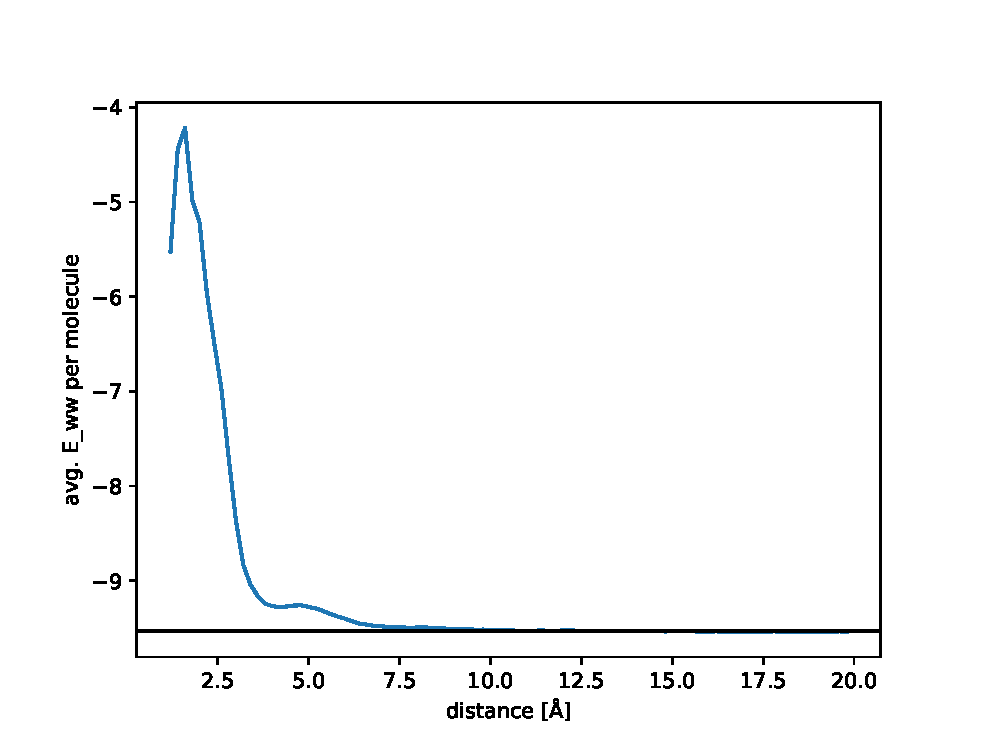
\includegraphics[width=0.8\linewidth]{figures/Eww_convergence.eps}
	\caption{Convergence of $E_{ww}$ with increasing distance to the solute. The horizontal line shows the automatically computed reference energy.}
	\label{fig_ewwref}
\end{figure}

\subsection{Visualizing $\dgsolv$}
\subsection{Contribution of Hydration to Binding}

%\section{Content and links}
%
%A tutorial will normally draw on additional files and materials; clearly indicate where and how these are available, with links, and how they are being archived for the long-term and maintained so they stay current.
%You will likely want to reference your GitHub repository as a central point to access all of this information, and then the GitHub repository may link out to other content as needed.

\section{Checklists}
%Tutorials do not necessarily require the use of a checklist as in Best Practices documents; however, they can include these if desired.
%Several useful checklist formats are available, with examples presented in \texttt{sample-document.tex} in \url{github.com/livecomsjournal/article_templates/templates}.
%One example is shown here.

% Here is a single-column checklist that consists of multiple sub-checklists
\begin{Checklists}

\begin{checklist}{Simulation settings}
\end{checklist}

\begin{checklist}{Obtaining absolute $\Delta G_\textup{solv}$ }
\end{checklist}

\begin{checklist}{A list}
\textbf{Single-column checklists are also straightforward by removing the asterisk}
\begin{itemize}
\item First thing let's do an item which breaks across lines to see how that looks
\item Also remember
\item And finally
\end{itemize}
\end{checklist}
%
%\begin{checklist}{Another list}
%\textbf{This is some further description.}
%\begin{itemize}
%\item First thing
%\item Also remember
%\item And finally
%\end{itemize}
%\end{checklist}

\end{Checklists}








\section*{Author Contributions}
%%%%%%%%%%%%%%%%
% This section mustt describe the actual contributions of
% author. Since this is an electronic-only journal, there is
% no length limit when you describe the authors' contributions,
% so we recommend describing what they actually did rather than
% simply categorizing them in a small number of
% predefined roles as might be done in other journals.
%
% See the policies ``Policies on Authorship'' section of https://livecoms.github.io
% for more information on deciding on authorship and author order.
%%%%%%%%%%%%%%%%

(Explain the contributions of the different authors here)

% We suggest you preserve this comment:
For a more detailed description of author contributions,
see the GitHub issue tracking and changelog at \githubrepository.

\section*{Other Contributions}
%%%%%%%%%%%%%%%
% You should include all people who have filed issues that were
% accepted into the paper, or that upon discussion altered what was in the paper.
% Multiple significant contributions might mean that the contributor
% should be moved to authorship at the discretion of the a
%
% See the policies ``Policies on Authorship'' section of https://livecoms.github.io for
% more information on deciding on authorship and author order.
%%%%%%%%%%%%%%%

(Explain the contributions of any non-author contributors here)
% We suggest you preserve this comment:
For a more detailed description of contributions from the community and others, see the GitHub issue tracking and changelog at \githubrepository.

\section*{Potentially Conflicting Interests}
%%%%%%%
%Declare any potentially competing interests, financial or otherwise
%%%%%%%

Declare any potentially conflicting interests here, whether or not they pose an actual conflict in your view.

\section*{Funding Information}
%%%%%%%
% Authors should acknowledge funding sources here. Reference specific grants.
%%%%%%%
FMS acknowledges the support of NSF grant CHE-1111111.

\section*{Author Information}
\makeorcid

\bibliography{bibliography}

%%%%%%%%%%%%%%%%%%%%%%%%%%%%%%%%%%%%%%%%%%%%%%%%%%%%%%%%%%%%
%%% APPENDICES
%%%%%%%%%%%%%%%%%%%%%%%%%%%%%%%%%%%%%%%%%%%%%%%%%%%%%%%%%%%%

%\appendix


\end{document}
